
%!TEX root = ../thesis.tex
%*******************************************************************************
%****************************** Third Chapter **********************************
%*******************************************************************************
\chapter{Calibration of Time Projection Chambers}
\label{ChapterCalib}
% **************************** Define Graphics Path **************************
\ifpdf
    \graphicspath{{Chapter8/Figs/Raster/}{Chapter8/Figs/PDF/}{Chapter8/Figs/}}
\else
    \graphicspath{{Chapter8/Figs/Vector/}{Chapter8/Figs/}}
\fi

%********************************** %Opening  **************************************
Calibrating the Time Projection Chamber (TPC) is a crucial step to study and correct for physics processes and detector effects impacting the deposited charges on wire planes.
Key processes affecting the production, propagation and detection of ionisation electrons are detailed in Chapter \ref{Chapter3}, including recombination, diffusion, electron attenuation and Space Charge Effect (SCE).
%of which electron attenuation and recombination are discussed in this chapter.
These effects have been well-studied by other LArTPC experiments like MicroBooNE \cite{uboone_calib, ubooneEtime}, ArgoNeuT \cite{argoneut_recomb}, and ICARUS \cite{icarus_recomb, GrayDiffusion}.
Their results have demonstrated an improvement in the spatial, temporal, and energy resolution of charge signals after correcting for these effects, demonstrating the importance of calibration to achieve high precision measurements.

Two Monte Carlo (MC) studies within the scope of charge calibration at the Short-Baseline Near Detector (SBND) are presented in this chapter, focusing on electron attenuation and recombination.
The first study of electron lifetime measurement is presented in Section \ref{sec7:etime}.
The second study is an assessment of the impacts of delta ray fluctuations on recombination, given in Section \ref{sec7:delta}.
Finally, Section \ref{sec:concludeDeltaRay} concludes the chapter with some remarks.

%with suggestions towards a data-driven calibration.
%suggestions for measurements that can carried out at SBND to improve and build toward a data-driven recombination model.
%Section \ref{sec7:etime_procedure} outlines a measurement procedure using an anode-to-cathode crossing cosmic track sample, whilst Section \ref{sec7:etime_bias} identifies detector effects that can introduce biases in the lifetime measurement.
%Improvements and updates on the procedure are summarised in Section \ref{sec7:etime_remark}.
%Section \ref{sec:simDeltaRay} details the simulation framework of delta rays and recombination.
%Section \ref{sec:impactDeltaRayMag} and \ref{sec:impactDeltaRaySmear} describe the impacts of delta rays on the magnitude and smearing of recombination respectively, while Section \ref{sec:impactStepLimit} examines the length scale of the simulation framework.
%to have a better understanding of the simulation framework for this phenomenon.

%********************************** %First Section  **************************************
\section{Electron Lifetime Measurement}
\label{sec7:etime}

Ionisation electrons can be captured by electronegative impurities present in liquid argon, as previously described in Section \ref{sec:edrift}.
The reduction of the number of charges collected on a wire can be modelled as an exponential decay function following Eq. \ref{eq:etime}, where the electron lifetime $\tau$ indicates the argon purity level of the detector.
A higher electron lifetime corresponds to a higher purity and vice versa.
The electron lifetime can be precisely measured and used to recover the original charge deposition on the wires.

At SBND, there are several methods to measure the electron lifetime.
Firstly, three purity monitors were installed, two inside the cryostat and one outside, which provide quick and real-time monitoring of the argon purity.
Another method requires a dedicated extraction of electron lifetime using deposited charges as measured by the wires.
This calibration procedure is often performed on a sample of cosmic muons that fully cross the drift distance of the TPC, known as \textit{anode-to-cathode} cosmic tracks.
Since they traverse the whole drift distance, they make a good sample to study the charge deposited per unit length $dQ/dx$ dependence on the drift distance.
The MicroBooNE experiment also employed the same anode-to-cathode-crossing cosmic tracks to study and correct for position- and time-dependent response of their TPCs\cite{uboone_calib}.

The study aims to develop a procedure to measure electron lifetime and investigate detector effects that can introduce biases in the measurement, such as diffusion and SCE.
Anode-to-cathode cosmic tracks were simulated to perform the lifetime measurement.
%MC samples of crossing cosmic tracks were simulated to perform the lifetime measurement.
The procedure for electron lifetime measurement is outlined in Section \ref{sec7:etime_procedure}, followed by Section \ref{sec7:etime_bias} describing biases in lifetime measurement due to detector effects.


\subsection{Electron Lifetime Extraction Procedure}
\label{sec7:etime_procedure}

The electron lifetime measurement requires information on the deposited charge per unit length $dQ/dx$ and the respective drift time $t_{drift}$ of that charge cluster arrive at the wire.
The charge reconstruction follows the workflow described in Section \ref{sec:reco_tpc}, whilst additional calculation is required to deduce the drift time.     
The drift time is defined as:
\begin{equation}
        t_{drift} = \frac{x}{v_{d}},
\end{equation}
where $x$ is the location the charge deposition in the drift direction ($x$-axis) and $v_{d}$ is the drift velocity.
At SBND, the drift velocity is expected to be at 0.1563 cm/$\mu$s at an electric field of 0.5 kV/cm and temperature of 88.4 K (See Section \ref{sec:edrift}).
The drift time can be calculated using the time recorded by the TPC readout when a charge cluster arrives at a wire $t_{m}$ which is defined as \cite{pandora_protodune}:
\begin{equation}
\label{eq:t0}
        t_{m} = t_{0} - t_{trigger} + t_{drift},
\end{equation}
where $t_{0}$ is the time when the particle enters the detector and $t_{trigger}$ is the time when the TPC readout is triggered.
For a beam neutrino that triggers the TPC readout, the readout window is configured to align with when the beam arrives at the detector such that $t_{trigger} = t_{0}$, as illustrated in Fig. \ref{fig:SBNDEventStructure} in Section \ref{sec:evb}.
On the other hand, a cosmic muon can occur anytime within the readout window and the time when it enters the detector $t_{0}$ is unknown.

A \textit{cathode stitching} process was developed by the ProtoDUNE and Pandora collaboration to determine the $t_{0}$ of cosmic muons that cross the cathode \cite{pandora_protodune}.
This can be applied to any LArTPC experiments that have two TPCs sharing the same cathode.
Fig. \ref{fig:cosmic_stitch} depicts the \textit{stitching} process.
The reconstruction algorithm begins with an initial and incorrect assumption of $t_{0} = 0$ \cite{pandora_protodune}, so that two cosmic track segments, shown by the red and blue lines, appear at the wrong positions in both drift volumes.
The algorithm then shifts the drift coordinate in each TPC by an equal and opposite amount until the two segments are \textit{stitched} at the cathode, shown by the black line, to recover the correct $t_{0}$.
This method has been implemented in the reconstruction workflow of SBND, and it was applied to reconstruct the sample of anode-to-cathode-crossing tracks in this study.
%Once $t_{0}$ is determined, the drift time can then be calculated using Eq. \ref{eq:t0}. 

\begin{figure}[h!] 
\centering    
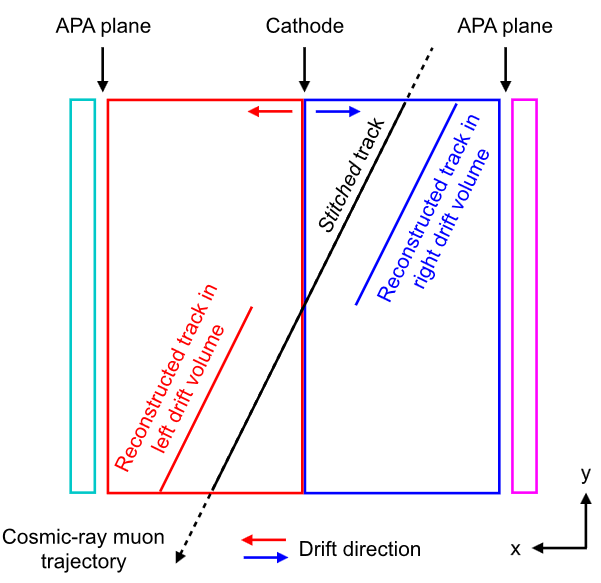
\includegraphics[width=0.55\textwidth]{cosmic_stitch}
\caption[Cathode Stitching Diagram]{
Cathode stitching process to determine the $t_{0}$ of cathode-crossing track \cite{pandora_protodune}.
}
\label{fig:cosmic_stitch}
\end{figure}

The next step in the lifetime extraction procedure was to plot the deposited charge per unit length $dQ/dx$ in bins of the drift time $t_{drift}$.
Fig. \ref{fig:dqdxMPV} shows an example $dQ/dx$ profile in the drift time bin from 0.925 to 0.95 ms.
A Landau-Gaussian convolution was fitted to the profile to extract the Most Probable Value (MPV) of $dQ/dx$ \cite{Passage}.
This process was repeated for every drift time bin across the full drift distance of the TPC.

Fig. \ref{fig:etime_tpc} shows the MPV $dQ/dx$ as a function of drift time, for TPC 0 (east) and 1 (west) of SBND.
Bins of drift time less than 0.25 ms and larger than 1.15 ms were excluded due to the close proximity to the anode and cathode respectively, which can introduce some boundary effects.
The MPV $dQ/dx$ distribution is fitted with Eq. \ref{eq:etime} to determine the electron lifetime constant.
The MC sample input to Fig. \ref{fig:etime_tpc} was simulated with a lifetime of 10 ms and no detector effects enabled to validate the procedure.                                       
The lifetimes were determined to be $10.12\pm0.24$ and $10.40\pm0.29$ ms, for TPC 0 and 1 respectively, showing a good agreement between the result and the simulation. 

\begin{figure}[hb!] 
\centering    
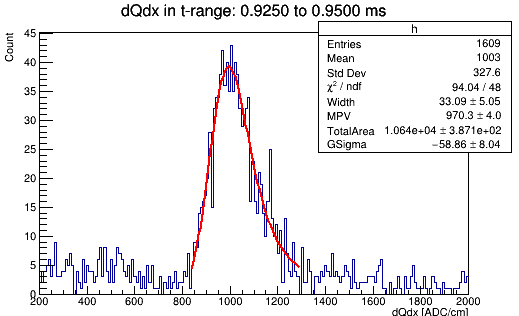
\includegraphics[width=0.55\textwidth]{dqdxMPV}
\caption[dQ/dx Profile Fitted With a Laundau-Gaussian]{
Example of a $dQ/dx$ profile in a drift time bin of 0.925--0.95 ms, fitted with a Landau-Gaussian convolution.
}
\label{fig:dqdxMPV}
\vspace{0.5cm}
%\end{figure}
%\begin{figure}[htbp!]
        \centering
        \begin{subfigure}[b]{0.495\textwidth}
            \centering
            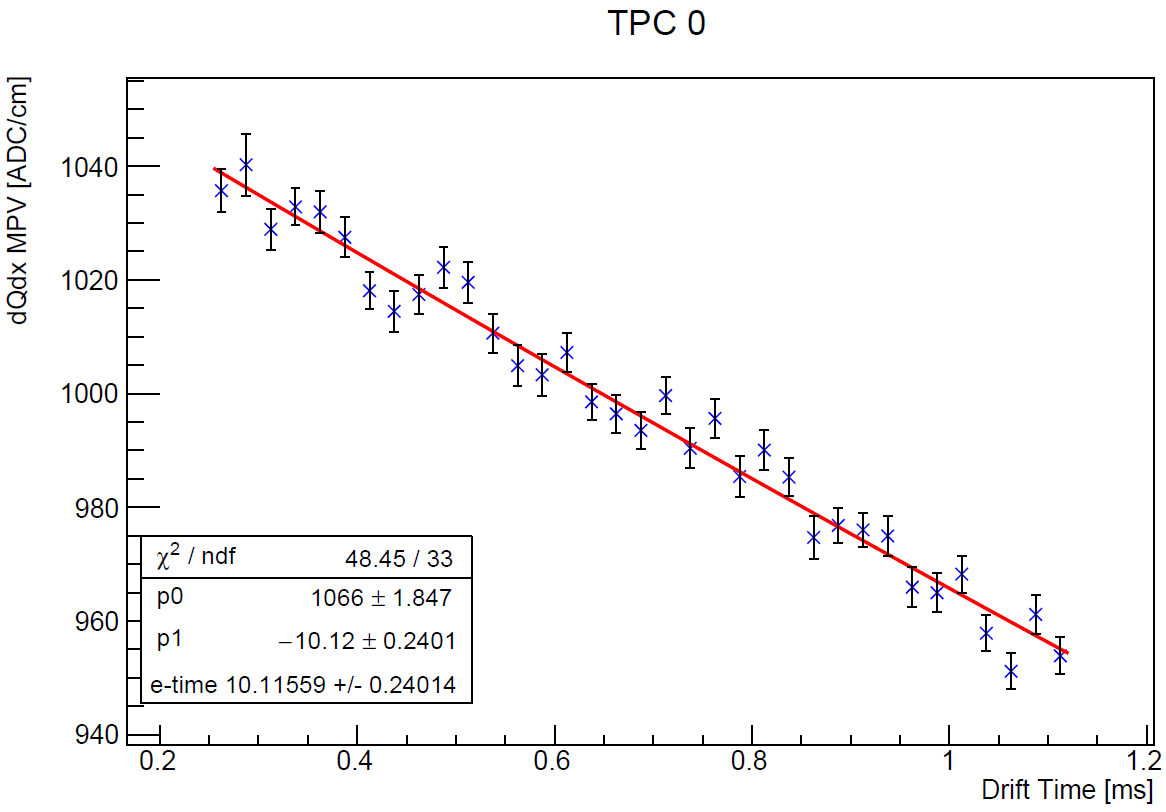
\includegraphics[width=\textwidth]{etime_tpc0}
            %\caption{}%
            %\label{}
        \end{subfigure}
        \hfill
        \begin{subfigure}[b]{0.495\textwidth}  
            \centering 
            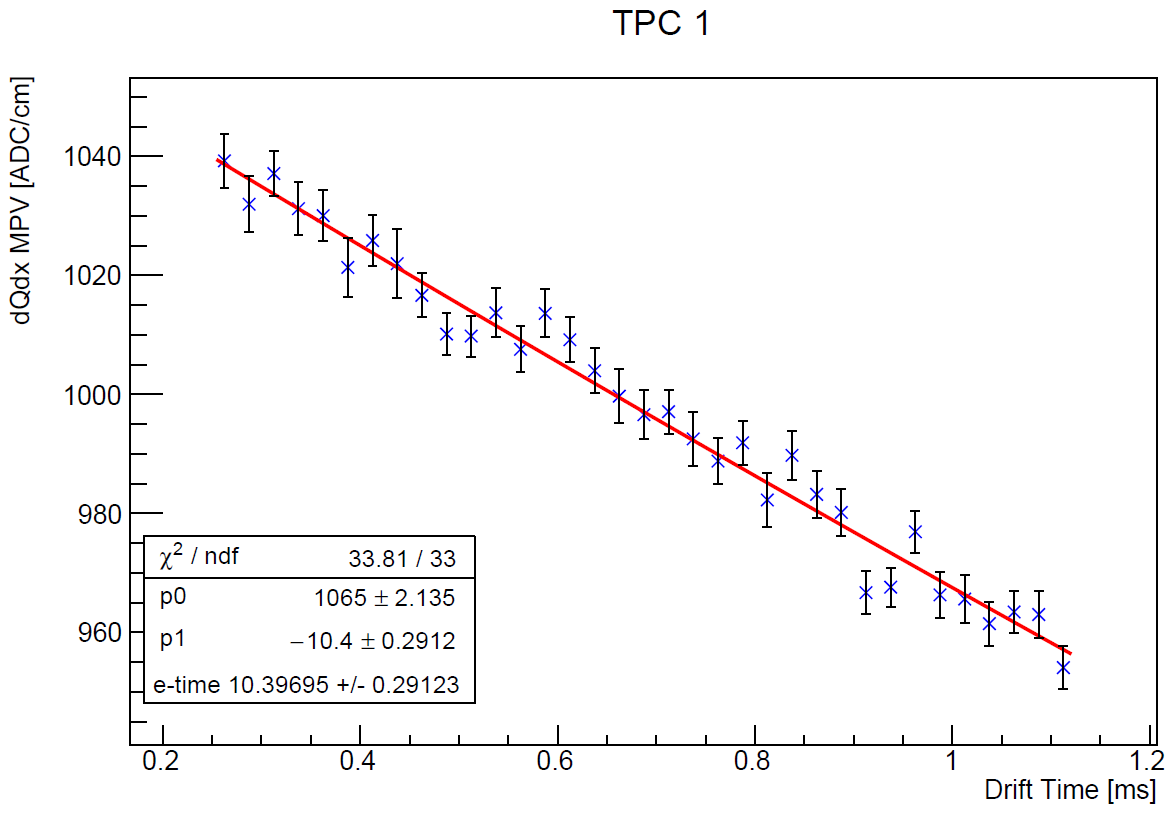
\includegraphics[width=\textwidth]{etime_tpc1}
            %\caption{}%
            %\label{}
        \end{subfigure}
        \caption[Most Probable Value dQ/dx Against Drift Time]{MPV $dQ/dx$ as a function of drift time, fitted with an exponential function.}
        \label{fig:etime_tpc}
\end{figure}

\subsection{Bias Study of Diffusion and Space Charge Effects}
\label{sec7:etime_bias}

Some detector effects can introduce biases to the electron lifetime measurement, specifically those that can influence the propagation path of drifting electrons such as diffusion and SCE.
Diffusion smears both spatial and temporal resolutions of the drifting electrons, and consequently the number of wires seen by the charge and the arrival time of charge measured by the wires.
SCE impacts both the amplitude of the deposited charge as well as the temporal and spatial resolution due to electric field distortion.
A study was undertaken to understand how each effect introduces biases to the measurement of electron lifetime.

Three dedicated MC samples were simulated: (1) No SCE nor diffusion enabled, (2) only diffusion enabled and (3) only SCE enabled.
In the diffusion-only MC sample, the longitudinal diffusion coefficient was set at $D_{L} = 4.0 $ cm$^{2}$/s, as measured by MicroBooNE \cite{uboone_diff}, and the transverse diffusion coefficient was set at $D_T = 8.8 $ cm$^{2}$/s, as measured by ProtoDUNE \cite{protodune} (See Section \ref{sec:edrift}).     
In the SCE-only MC sample, the simulation of electric field distortion followed the description in Ref. \cite{SCE}.
%The electron lifetime was measured for each sample.

Biases in the lifetime compared to the simulated lifetime are shown in Fig. \ref{fig:etime_biases_compare}, for two simulated electron lifetimes at 3 ms (top) and 10 ms (bottom).
When no detector effects are enabled in the simulation, the determined lifetimes are very similar to the simulated lifetimes, with biases well below the 2\% level.
When either diffusion or SCE was enabled in the simulation, biases in the lifetimes can be seen.
Biases due to diffusion are at $\sim 2\%$ and $\sim 4\%$ for the simulated lifetimes of 3 ms and 10 ms respectively.
On the other hand, biases due to SCE are higher at $\sim 5 \%$ and $\sim22 \%$ at the simulated 3 ms and 10 ms lifetime.
The observed biases are also consistent across the two TPC volumes of SBND.

The first observation is that the magnitude of the biases due to SCE is much greater than due to diffusion at both simulated lifetimes.
This is consistent with the observations from an electron lifetime measurement carried out by MicroBooNE \cite{ubooneEtime}. 
The paper demonstrated that both SCE and the transverse component of diffusion cause biases in the lifetime, however, biases due to transverse diffusion are smaller in magnitude than SCE.
The paper also pointed out that the longitudinal component of diffusion causes insignificant biases in the lifetime.

The second observation is that the longer the lifetime, the larger the biases as compared between the lifetimes at 3 ms and 10 ms.
This is most likely due to the precision of this method worsening with increasing lifetimes.
Larger lifetime leads to a more uniform $dQ/dx$ distribution across the drift distance, and thus, fitting an exponential function can become less reliable.
%This is due to more drifting electrons surviving with a larger lifetime and thus, becoming more susceptible to detector effects.

\begin{figure}[t!] 
\centering    
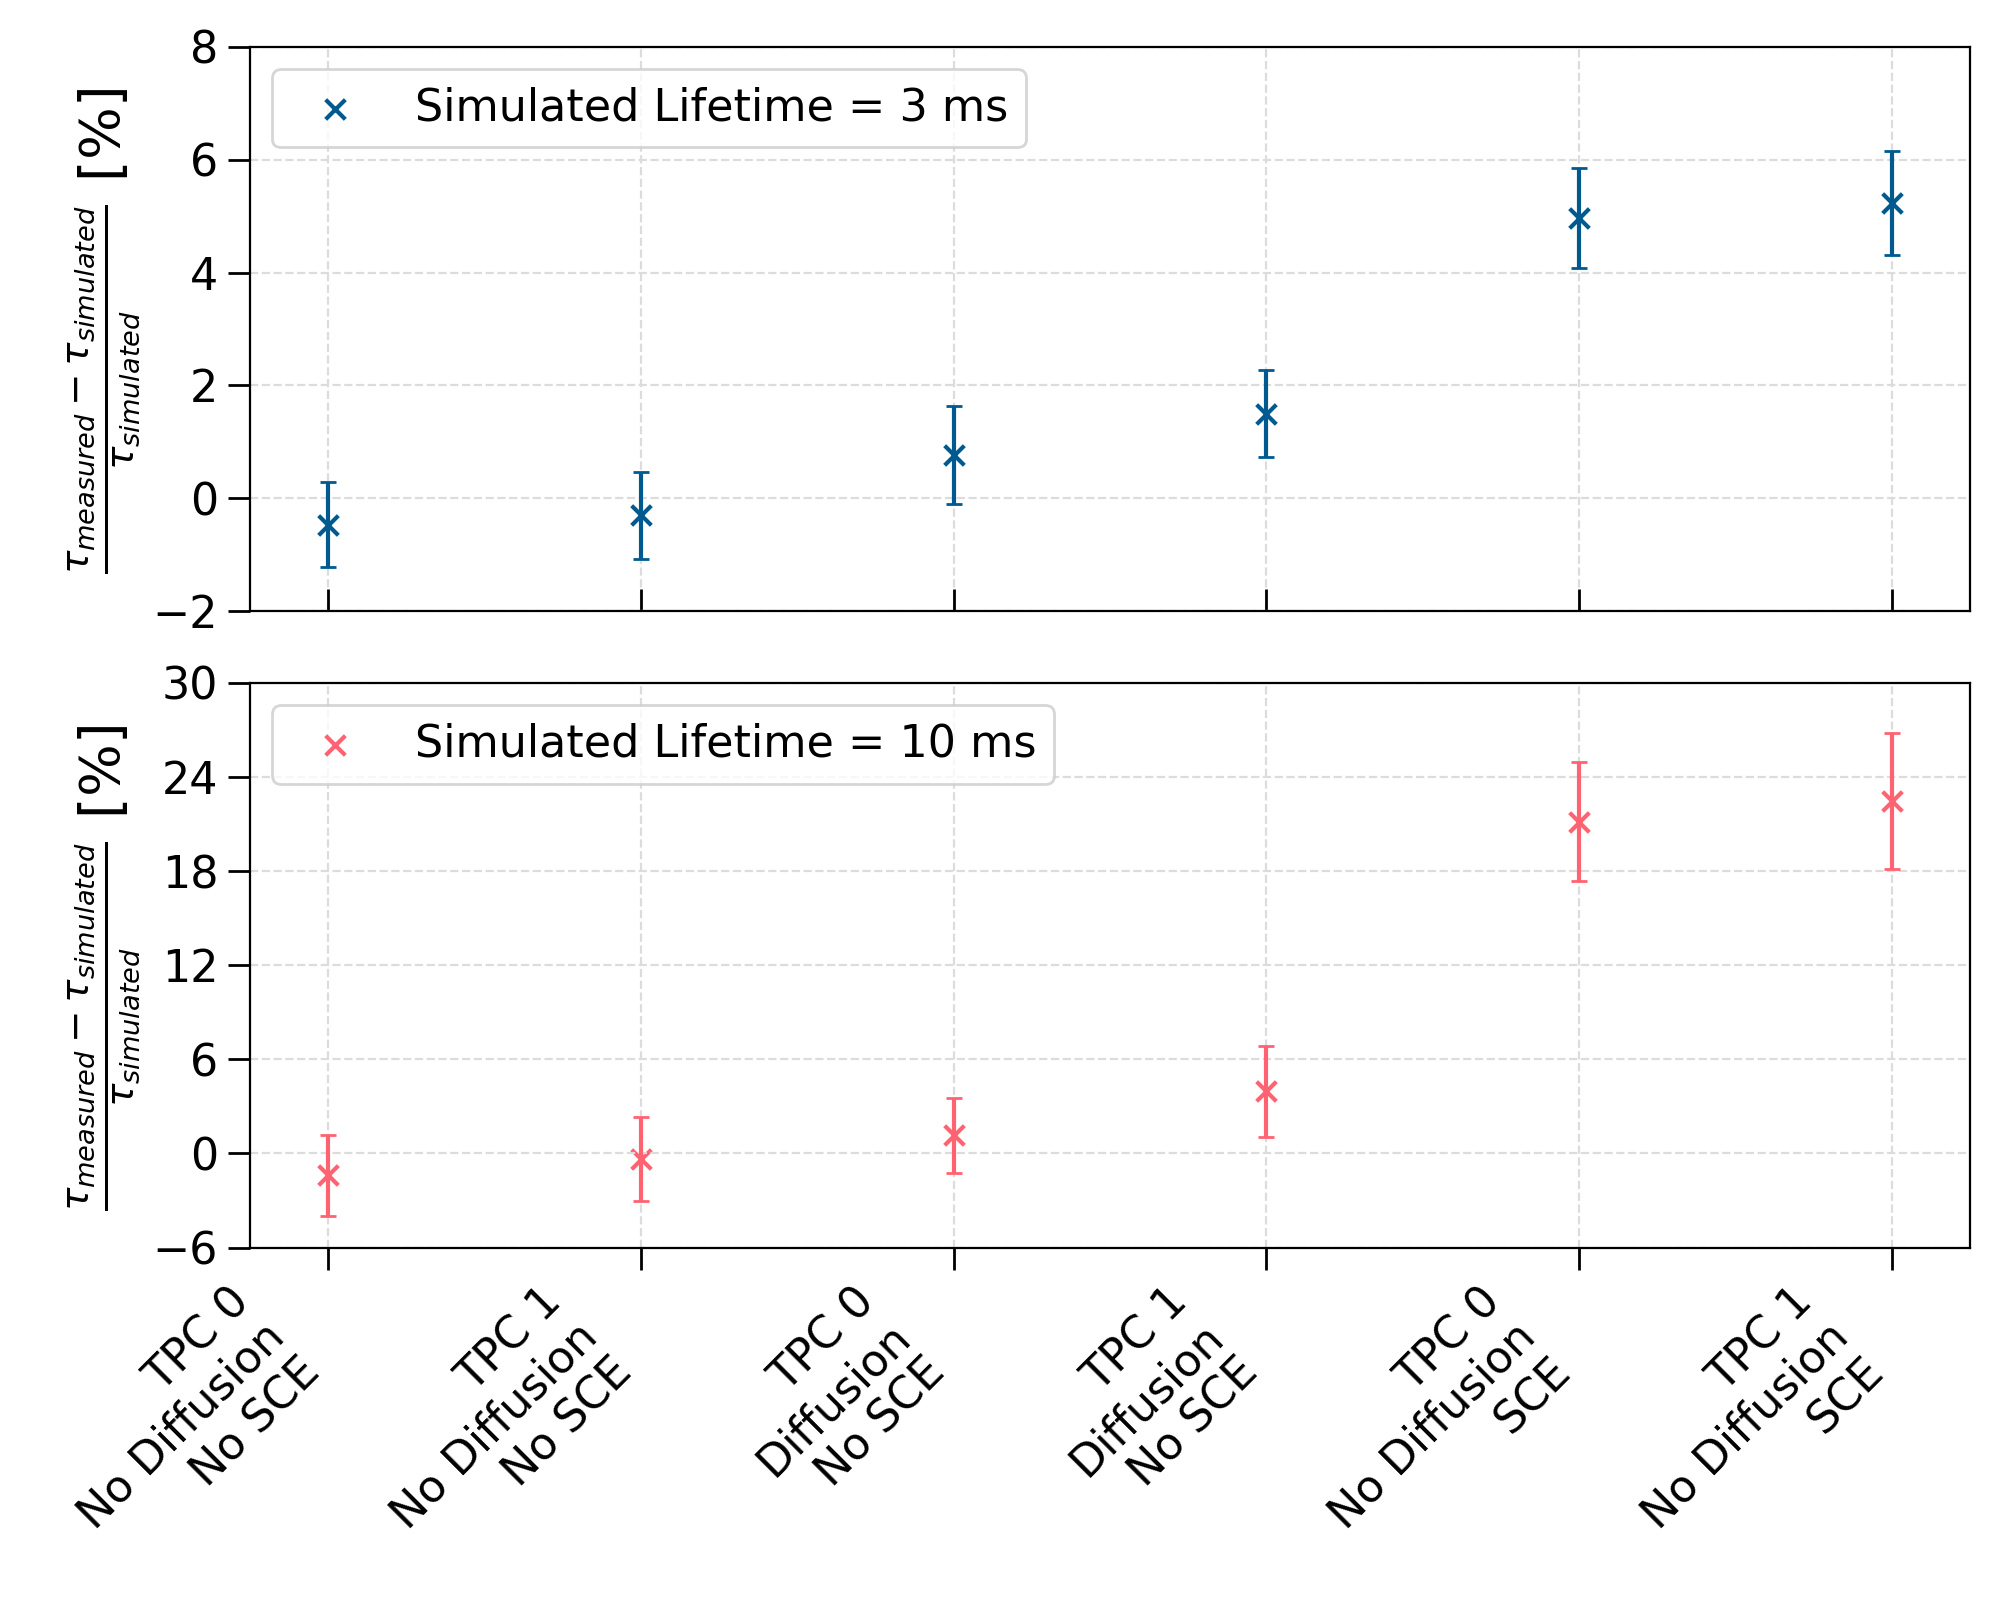
\includegraphics[width=0.85\textwidth]{etime_biases_compare}
\caption[Electron Lifetime Measurement Biases]{
Biases in electron lifetimes compared to the simulated values at 3 ms (top) and 10 ms (bottom).
}
\label{fig:etime_biases_compare}
\end{figure}

Since the results of this study, an investigation at the ICARUS experiment demonstrated that transverse diffusion breaks down the Landau-Gaussian MPV approximation of the measured charge \cite{GrayDiffusion}, which was employed in this study.
This is due to transverse diffusion smearing the charge cluster across multiple wires, resulting in a shift in the MPV value. 
The paper recommends using an averaged $dQ/dx$ from a group of wires instead of $dQ/dx$ from a single wire to mitigate the effect.
The suggestion has been implemented at SBND.

The study presented here demonstrates a method to measure electron lifetime using a sample of anode-to-cathode crossing cosmic tracks.
These tracks have the advantage of spanning over a full drift distance and a reconstructable $t_{0}$ time tagging when the particle enters the detector.
The electron lifetime measured by this method is the most affected by SCE, followed by diffusion, which is consistent with the results from MicroBooNE.
This procedure has now been replicated in preparation for the calibration run of SBND at the time of writing.
A trigger requiring coincidence in the east and west CRT wall was deployed to produce dedicated samples containing crossing cosmic muon tracks that can be used for electron lifetime measurement.

%********************************** %First Section  **************************************

\section{Delta Ray Fluctuations on Recombination}
\label{sec7:delta}

%As discussed in Chapter \ref{ChapterSim}, simulation plays a vital role in neutrino physics.
%The need to correctly simulate physics processes must be addressed to validate against data and build towards a data-driven simulation.
%The physics process of this simulated study is recombination, which drives the charge and light yield.                                              
%and tuned for simulation to match data .
%., as some additional charges of the track itself

%Introduce why this is important
Recombination is a physics process that drives the charge and light yield as previously described in Section \ref{sec:recomb}.
SBND currently employs the Modified Box (ModBox) model for simulating recombination, with experimentally-derived parameters from ArgoNeuT \cite{argoneut_recomb}.
The model approximates the recombination probability based on a cylindrical column surrounding a track-like charge deposition, effectively accounting for microphysics processes along the track.
This approximation has proven to work well for the MeV to GeV-scale interactions, however, it breaks down at the keV-scale.

%The NEST collaboration pointed out non-linear fluctuations in recombination at increasingly smaller scales that are not well-described by the ModBox model \cite{NEST}.   
%Moreover, the ArgoNeuT collaboration also proposed that microphysics effects could lead to disagreements in recombination theory and data \cite{argoneut_recomb}.

Delta rays are microphysics processes that can affect recombination, highlighted by both NEST \cite{NEST} and ArgoNeuT \cite{argoneut_recomb} collaborations.
They are knock-out electrons with low energy but high energy loss per unit length $dE/dx$.
As shown in Fig. \ref{fig:delta_ray_evd}, delta rays are short blip produced along a longer primary track, in this case, a cosmic muon.                      
Due to their high $dE/dx$, they are associated with a smaller recombination factor $R$ (See Fig. \ref{fig:recomb_graph} Section \ref{sec:recomb}).
A smaller $R$ corresponds to a smaller probability of ionisation electrons surviving recombination.
As a result, delta rays can lead to non-linear fluctuations in recombination that is not well-described by the ModBox model.
%to higher recombination, producing more scintillation photons at the cost of ionisation electrons.

This study is motivated to asses the impacts of delta ray fluctuations on recombination, and consequently, the charge to energy loss conversion of different particle types using MC.
An overview of the simulation of delta rays and recombination is given in Section \ref{sec:simDeltaRay}.%, and some concerns with the current framework.
Following this, Sections \ref{sec:impactDeltaRayMag} and \ref{sec:impactDeltaRaySmear} provide a description of the delta ray impacts on the recombination magnitude and smearing respectively.
A summary of recombination studies carried out by the ICARUS collaboration is given in Section \ref{sec:icarus}.

\begin{figure}[hb!] 
\centering    
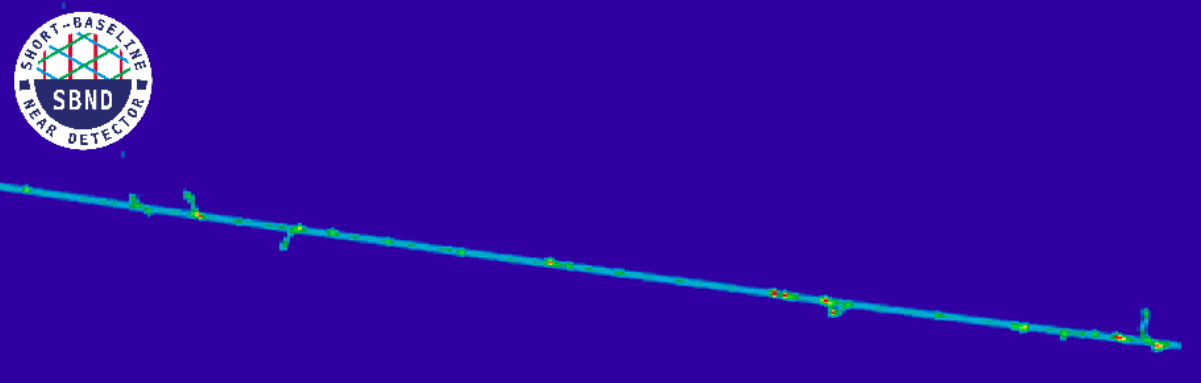
\includegraphics[width=0.85\textwidth]{delta_ray_evd}
\caption[Event Display of a Cosmic Muon and Delta Rays]{
Event display of a simulated cosmic muon track segment, with many delta rays produced along the track.
}
\label{fig:delta_ray_evd}
\end{figure}

%Section \ref{sec:impactDeltaRayMag}, \ref{sec:impactDeltaRaySmear} and \ref{sec:impactStepLimit} describe the impacts of varying different simulation handles associated with delta rays on particle calorimetry.
%Finally, Section \ref{sec:concludeDeltaRay} suggests recommendations for measurements at SBND to improve the recombination model.             

\subsection{Simulation of Delta Rays and Recombination}
\label{sec:simDeltaRay}

Delta rays and recombination are simulated as part of the particle propagation simulation performed by the Geant4 toolkit \cite{geant4}, with details provided in Section \ref{sec:gen_g4}.
The simulation propagates the primary particle step by step and applies physics processes at each step of length $dx$.
Particularly, this study focuses on the energy loss due to ionisation.
It is simulated as two dependent processes: (1) a continuous energy loss $dE$ of the primary particle along the step $dx$ and (2) a discrete energy loss $dE$ at the end of the step producing delta rays \cite{geant4}.

The continuous energy loss of the primary particle is simulated by Geant4 using complementary models depending on the particle Kinetic Energy (KE) \cite{geant4_ions}.
For particles with KE > 2 MeV, the Bethe-Bloch formalism \cite{Passage}, detailed in Section \ref{sec3:bethebloch}, is used to compute the mean $dE/dx$.
In the intermediate KE range range < 2 MeV, simulation models parameterised on data from Ref. \cite{Ziegler} and Ref. \cite{ICRU} are implemented.
In the low KE < 1 keV, Geant4 uses the free electron gas model since no data is available.

%the total cross section of the delta ray production 
The discrete energy loss to produce delta rays is determined by a user-defined energy threshold.
The energy threshold defines the lower limit of the KE of delta rays so that only delta rays with sufficient energy can be produced.
This is to suppress the simulation of all low energy delta rays that would exhaust computation resources.
This also means that the energy of the non-produced delta rays is transferred to the continuous energy loss of the primary particle.
This is equivalent to setting the energy threshold as the upper limit for the primary particle so that its mean continuous energy loss is less than the threshold.
%In other words, the energy threshold determines how much energy deposition is shared between the primary particle and the delta rays. 
%The lower the threshold, the more energy deposition is carried away by the delta rays instead of the primary particle. 

In Geant4 terminology, the energy threshold is also known as the secondary production threshold, where the minimum KE requirement for delta ray production is defined as the minimum distance the generated delta ray must be able to traverse in a given material. 
These thresholds will be referred to as \textit{delta ray thresholds} in short from this point onwards in this study. 
Moreover, the maximum length $dx$ that the particle can propagate per step is configured as 0.3 mm, one order of magnitude smaller than the wire pitch of 3 mm.
This setup allows for a feasible computation of generating delta rays.

%Describe ionandscint module
For each step $dx$, the number of electron-ion pairs resulting from a continuous loss energy deposition $dE$ is calculated by dividing $dE$ by the ionisation work function of argon $W_{ion} = 23.6$ eV \cite{wion_lar}.
Recombination factor $R$ is applied to the number of electron-ion pairs according to the charge-light anti-correlation described by Eq. \ref{eq:Q} and \ref{eq:L} to determine the number of surviving electrons resulting from the step $dx$.    
Using the ModBox formalism, $R$ is computed as \cite{argoneut_recomb}:
\begin{equation}
        \label{eq:R_factor}
        R = \frac{\log{ \left( \alpha + \left(\beta \cdot dE/dx\right)/\varepsilon \right)}}{\left(\beta \cdot dE/dx\right)/\varepsilon},
\end{equation}
where $\varepsilon$ (kV/cm) is the electric field at the position of the step, $dE/dx$ (MeV/cm) is the energy loss per unit length, and parameters $\alpha = 0.93\pm0.02$ and $\beta = 0.212\pm0.002$ (kV/cm
)(g/cm$^{2}$)/MeV were experimentally derived by ArgoNeuT \cite{argoneut_recomb}.
Eq. \ref{eq:R_factor} is plotted in Fig. \ref{fig:recomb_graph} in Section \ref{sec:recomb}.
It is important to note that $R$ is dependent on the electric field and therefore can be influenced by local distortions of the field.

%potential issue
The simulation of delta rays and recombination described here gives rise to some concerns.
The first concern is the assumption of a \textit{universal} recombination factor $R$.
The parameters $\alpha$ and $\beta$ were measured by ArgoNeuT using a stopping proton sample, and wire planes with a pitch of 3 mm \cite{argoneut_recomb}.
Nonetheless, they are applied to any type of ionising particles, which can influence the local ionisation density differently. 
Secondly, the delta ray thresholds remove low energy electrons in simulation.
However, they are produced in reality and can affect recombination at a local scale. 
%Finally, the step length $dx$ is simulated at one order of magnitude smaller than the wire pitch of both ArgoNeuT and SBND.

%how to validate
The study was set up to address the individual concerns outlined above to better understand their impacts on recombination.
Identical MC samples of muons and protons were simulated to investigate if recombination is particle-dependent.
The particles were generated with a fixed energy of 1 GeV, uniform in positional and angular distributions.
The Geant4 simulation was configured such that the particle can only deposit energy via ionisation.
The \textit{true} energy loss per unit length $dE/dx$ was computed from the \textit{true} number of electrons per unit length $dQ/dx$, where \textit{true} indicates no detector simulations were applied. 
The computation follows the ModBox formalism for charge to energy loss conversion as \cite{argoneut_recomb}:
\begin{equation}
        \label{eq:recomb_modbox}
        \frac{dE}{dx} = \frac{1}{\beta}\left[ \exp{\left( \beta W_{ion}  \frac{dQ}{dx}\right)} -\alpha \right],
\end{equation}
where parameters are the same as Eq. \ref{eq:R_factor}.
For each particle type, a range of delta ray thresholds were simulated.
The largest value, and also the current value being used by SBND, was set at 700 $\mu$m, equivalent to delta rays with a minimum KE of 273 keV.
The smallest threshold was 1 $\mu$m, enabling the simulation of delta rays with KE as low as 1 keV.
This variation was chosen to study the impacts due to delta ray fluctuations.

%was performed by reconstructing deposited energy $dE/dx$ from charge $dQ/dx$ collected on collection planes using Eq. \ref{eq:recomb_modbox}.
%A comparison was carried out on two identical samples of muons and protons using $true$ variables, to investigate if recombination is particle-dependent.
%Recombination is highly dependent on the electric field and the local charge density, and therefore a parameter for the electric field is folded into the $\beta$ parameter.

%
%, and formally modelled as follows \cite{argoneut_recomb}
%\begin{equation}
%	R=W_{ion} \cdot \frac{dE/dx}{dQ/dx}
%	\label{eq:recomb}
%\end{equation}
%where $W_{ion} = 23.6$ eV is the energy required to ionise an argon \cite{ion_e} and $dQ/dx$ and $dE/dx$ is the charge and energy loss per unit length respectively. 
%$W_{ion} = 23.6\pm0.3$ eV \cite{wion_lar} is the ionisation work function in argon 
%By re-arranging Eq. \ref{eq:recomb_modbox}, the recombination factor $R$ as a function of $dE/dx$ is derived as
%where .

\subsection{Impacts of Delta Rays on Recombination Magnitude}
\label{sec:impactDeltaRayMag}

Fig. \ref{fig:proton_2d} shows the simulated charge to energy loss conversion, $dQ/dx$ to $dE/dx$, for protons at the delta ray threshold of 700 $\mu$m and 1 $\mu$m.
The distribution was plotted for the proton residual range from 1 cm to 90 cm to cover the full track length. 
The proton $dE/dx$ ranges from 2 MeV/cm to 18 MeV/cm, allowing for the examination of delta ray fluctuation impacts at both low and high parts of the $dE/dx$ spectrum. 
For the delta ray threshold of 700 $\mu$m shown in Fig. \ref{fig:proton_2d_700}, the distribution precisely follows the ModBox model with the ArgoNeuT parameters defined in Eq. \ref{eq:recomb_modbox}.
A good agreement is expected since the simulation of SBND is similar to that of ArgoNeuT \cite{argoneut_recomb}.
%: (1) the maximum step length $dx$ was restricted to be 0.3 mm and (2) the energy loss due to delta rays was not included in recombination.

However, for the delta ray threshold of 1 $\mu$m shown in Fig. \ref{fig:proton_2d_1}, deviations away from the ModBox model occur, such that the distribution shifts at both low and high parts of the $dE/dx$ specturm. 
Lowering the delta ray threshold leads to more energy loss carried by the delta rays instead of the primary proton, and thus, delta rays have a greater influence on recombination.
At the low $dE/dx$ spectrum of the proton, delta rays have higher $dE/dx$ and a smaller recombination factor $R$ than that of the proton.
This results in the \textit{effective recombination factor} being reduced, decreasing $dQ/dx$ at the same value of $dE/dx$. 
The opposite effect is seen at the high $dE/dx$ spectrum of the proton, where $dQ/dx$ is higher than the ModBox model.
This indicates that the effective recombination factor increases, accounting for both the primary proton and delta rays.

%impacts from delta rays fluctuations on the charge to energy loss conversion. 

\begin{figure}[ht!]
        \centering
        \begin{subfigure}[b]{0.495\textwidth}
            \centering
            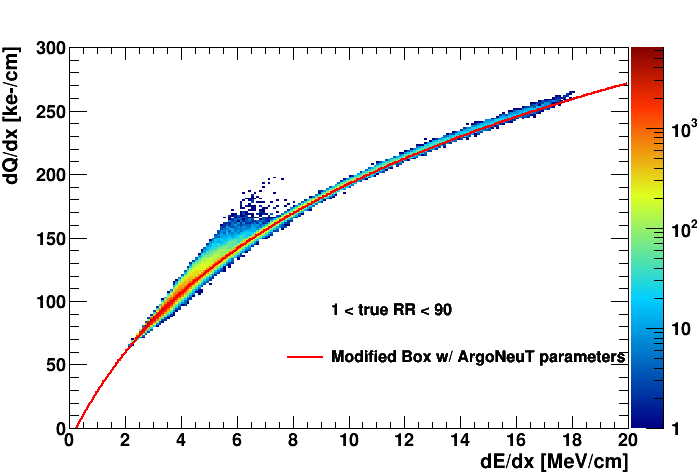
\includegraphics[width=\textwidth]{proton_700um}
            \caption{700 $\mu$m}%
            \label{fig:proton_2d_700}
        \end{subfigure}
        \hfill
        \begin{subfigure}[b]{0.495\textwidth}  
            \centering 
            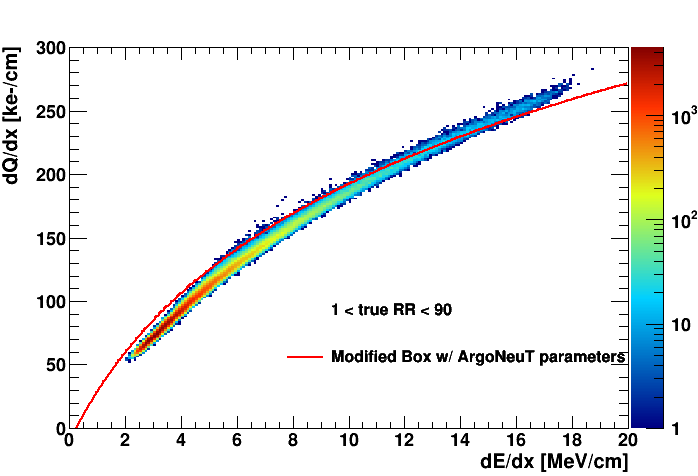
\includegraphics[width=\textwidth]{proton_1um}
            \caption{1 $\mu$m}%
            \label{fig:proton_2d_1}
        \end{subfigure}
	\caption[Charge to Energy Loss Conversion of a 1 GeV Proton]{$dQ/dx$ as a function of $dE/dx$ for a 1 GeV proton at the delta ray threshold of (a) 700 $\mu$m and (b) 1 $\mu$m.}
        \label{fig:proton_2d}
%\end{figure}
%\begin{figure}[htbp!]
        \begin{subfigure}[b]{0.495\textwidth}   
            \centering 
            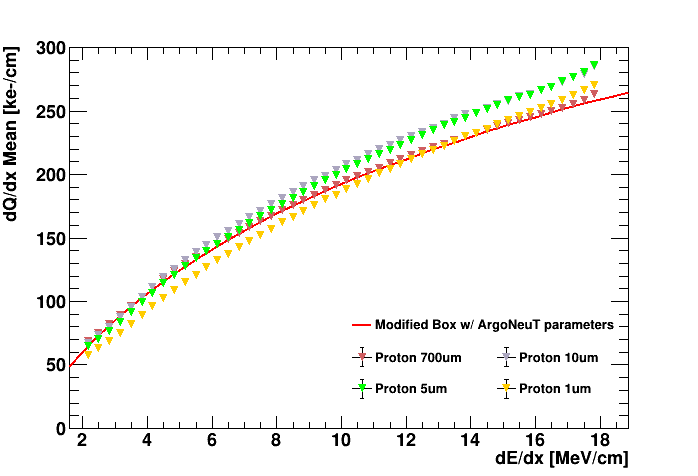
\includegraphics[width=\textwidth]{proton_profile}
            \caption{}%
            \label{fig:proton_range_delta_magnitude}
        \end{subfigure}
        \hfill
        \begin{subfigure}[b]{0.495\textwidth}   
            \centering 
            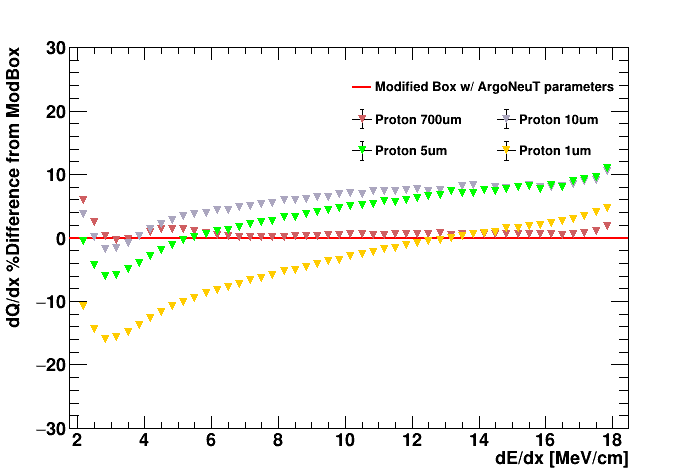
\includegraphics[width=\textwidth]{proton_profile_diff}
            \caption{}%
            \label{fig:proton_range_delta_diff}
        \end{subfigure}
	\caption[Impacts of Delta Ray Fluctuations on Protons]{(a) Mean $dQ/dx$ and (b) its percentage difference relative to the ModBox model as a function of $dE/dx$ for a 1 GeV proton. }
        \label{fig:proton_range_delta}
\end{figure}

%This then allows the determination of the output simulated recombination factor, given as $dE/dx / (W \times dQ/dx)$.
The proton charge to energy loss conversion at the thresholds of 700, 10, 5, and 1 $\mu$m, equivalent to delta rays with a minimum KE of 272.58, 14.60, 2.58, 1.06, and 0.99 keV are shown in Fig. \ref{fig:proton_range_delta}. 
To compare $dQ/dx$ quantitatively at the same $dE/dx$ bin, the mean $dQ/dx$ was calculated per $dE/dx$ bin as shown in Fig. \ref{fig:proton_range_delta_magnitude}.
The percentage difference of the mean $dQ/dx$ relative to the ModBox model is depicted in Fig. \ref{fig:proton_range_delta_diff} to quantify the magnitude of the differences.

Lowering the KE of delta rays results in two key trends.                                                         
Firstly, the $dE/dx$ position at which the proton charge to energy loss conversion shifts in upward/downward directions, increases with lower delta ray KE. 
This shift position can be seen in Fig. \ref{fig:proton_range_delta_diff}.
Secondly, the magnitude of the deviations depends on the delta ray threshold. 
At low $dE/dx < \sim 8$ MeV/cm, the effective recombination is reduced the most at the 1 $\mu$m threshold, as shown in yellow.
At high $dE/dx > \sim 8$ MeV/cm, the effective recombination is the highest at the 5 $\mu$m threshold, as shown in green.
This is evidence that delta ray fluctuations can greatly influence the proton charge to energy loss conversion.
The more energy loss is carried away by very low KE delta rays, the more distorted the charge to energy scale becomes.

%The linear distribution is due to the dressing the primary muon with very high energy delta rays, which have a linear charge to energy loss conversion. 
%This result in this linear feature that has been well observed experimentally with MIP muons. 

The charge to energy loss conversion for muons is plotted in Fig. \ref{fig:muon_2d}, for the delta ray threshold at 700 $\mu$m and 1 $\mu$m.
Fig. \ref{fig:mu_2d_700} and \ref{fig:mu_2d_1} contain the full muon residual range, covering the track length 1--400 cm.
Two distinct distributions can be seen here, one linear from the Minimum Ionising Particle (MIP) region, and another one that follows the ModBox model indicating the stopping region. 
The linear charge to energy loss conversion of MIP muons has been well-observed by LArTPC experiments, including MicroBooNE \cite{uboone_calib} and ICARUS \cite{icarus_recomb}.

To examine only the stopping region, a residual range requirement of less than 10 cm was applied, as shown in Fig. \ref{fig:mu_2d_700_lowRR} and \ref{fig:mu_2d_1_lowRR}.
The effects of lowering the delta ray can be seen by comparing the two figures. 
The same behaviour as protons at the same low $dE/dx$ $<\sim8$ MeV/cm is observed, where low energetic delta rays result in a smaller effective recombination factor, reducing $dQ/dx$ at the same value of $dE/dx$.

%Although, some remnants from the MIP region remains in the .
%between Fig. \ref{fig:mu_2d_700_lowRR} and \ref{fig:mu_2d_1_lowRR}.

\begin{figure}[b!]
        \centering
        \begin{subfigure}[b]{0.495\textwidth}
            \centering
            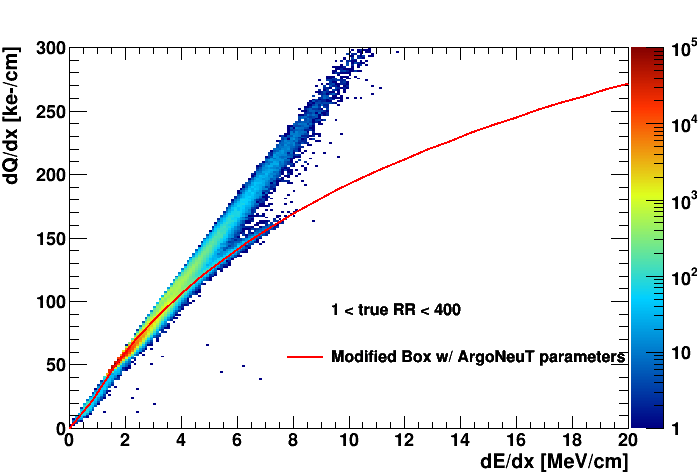
\includegraphics[width=\textwidth]{mu_700um}
            \caption{700 $\mu$m and full residual range}%
            \label{fig:mu_2d_700}
        \end{subfigure}
        \hfill
        \begin{subfigure}[b]{0.495\textwidth}  
            \centering 
            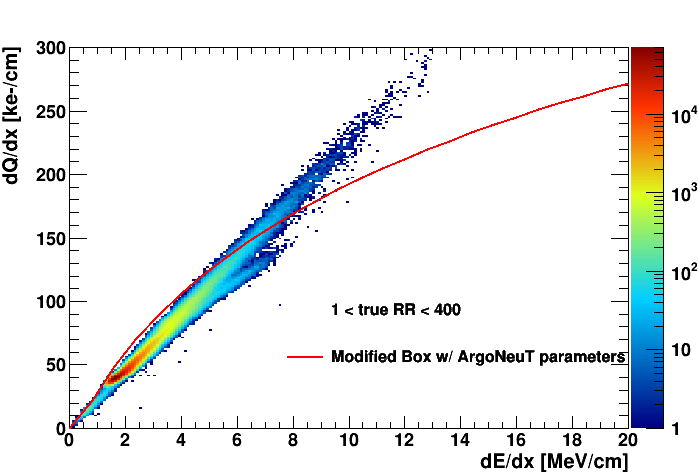
\includegraphics[width=\textwidth]{mu_1um}
            \caption{1 $\mu$m and full residual range}%
            \label{fig:mu_2d_1}
        \end{subfigure}
        %\vskip\baselineskip
        \begin{subfigure}[b]{0.495\textwidth}   
            \centering 
            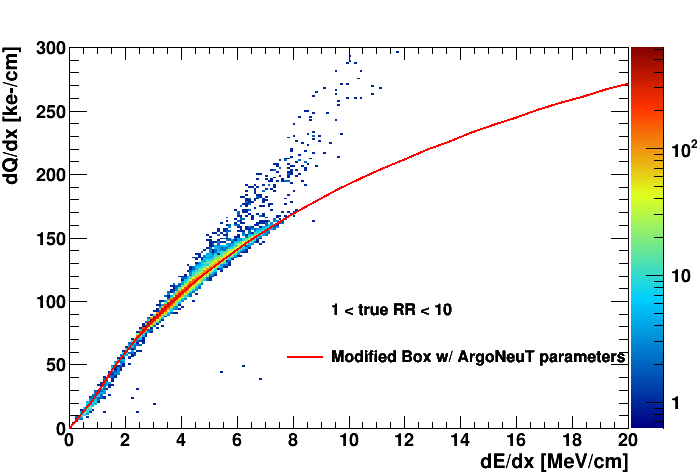
\includegraphics[width=\textwidth]{mu_700um_lowRR}
            \caption{700 $\mu$m and only stopping range}%
            \label{fig:mu_2d_700_lowRR}
        \end{subfigure}
        \hfill
        \begin{subfigure}[b]{0.495\textwidth}   
            \centering 
            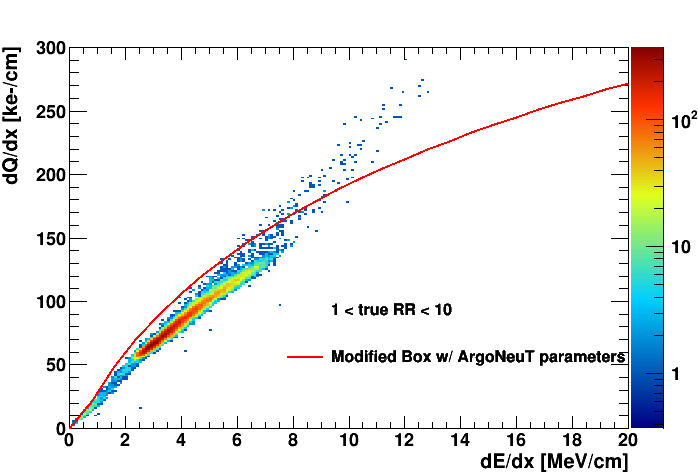
\includegraphics[width=\textwidth]{mu_1um_lowRR}
            \caption{1 $\mu$m and only stopping range}%
            \label{fig:mu_2d_1_lowRR}
        \end{subfigure}
	\caption[Charge to Energy Loss Conversion of a 1 GeV Muon]{
        	$dQ/dx$ as a function of $dE/dx$ for a 1 GeV muon at the delta ray threshold of 700 $\mu$m (left) and 1 $\mu$m (right) and for the full residual range (top) and only the stopping range (bottom).
	}
        \label{fig:muon_2d}
\end{figure}

The mean $dQ/dx$ of muons and its percentage difference relative to the ModBox model are also shown in Fig. \ref{fig:mu_range_delta}, at various values of delta thresholds.
Similar to protons, the effective recombination reduces with lower delta ray KE.
The recombination factor is also the most affected at the threshold of 1 $\mu$m, as shown in red.
It is also important to note that the magnitude of the reduction is larger for muons compared to protons, which is likely due to the amount of delta rays produced by each particle type.
For instance, at the same $dE/dx$ of 3 MeV/cm and the delta ray threshold of 1 $\mu$m, the percentage difference is at $\sim 24\%$ for muons and $\sim16\%$ for protons.  

The study demonstrates that fluctuations of delta rays can affect recombination.
Delta rays have a different $dE/dx$ compared to the primary particle and therefore, can influence the effective recombination factor.
At low $dE/dx$ $< \sim 8$ MeV/cm, this results in a reduction of the effective recombination accounting for both the primary particle and delta rays.
Meanwhile, at high $dE/dx$ $> \sim 8$ MeV/cm, delta rays can increase the effective recombination factor.
This leads to a distortion of the observed charge to energy loss conversion of a particle. 
The magnitude of the distortion is more significant for muons than protons.

\begin{figure}[t!]
        \begin{subfigure}[b]{0.495\textwidth}   
            \centering 
            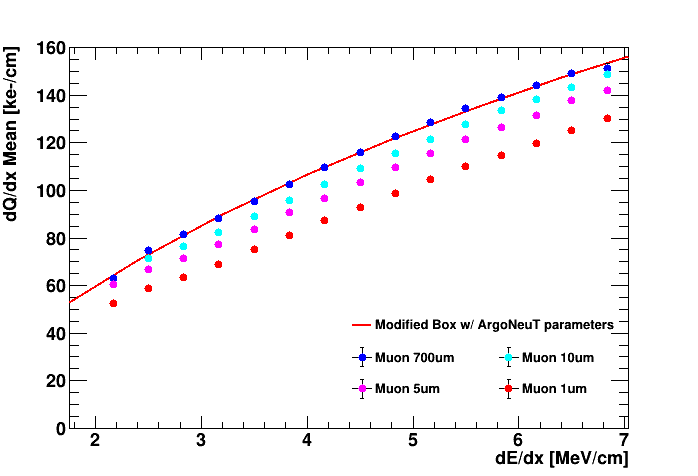
\includegraphics[width=\textwidth]{mu_profile}
            \caption{}%
            \label{fig:mu_range_delta_magnitude}
        \end{subfigure}
        \hfill
        \begin{subfigure}[b]{0.495\textwidth}   
            \centering 
            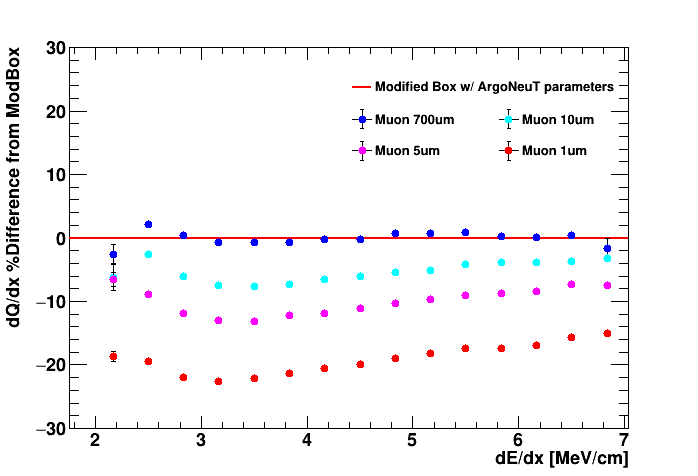
\includegraphics[width=\textwidth]{mu_profile_diff}
            \caption{}%
            \label{fig:mu_range_delta_diff}
        \end{subfigure}
	\caption[Impacts of Delta Ray Fluctuations on Muons]{(a) Mean $dQ/dx$ and (b) its percentage difference relative to the ModBox model as a function of $dE/dx$ for a 1 GeV muon. }
        \label{fig:mu_range_delta}
\end{figure}

\subsection{Impacts of Delta Rays on Recombination Smearing}
\label{sec:impactDeltaRaySmear}

%The effects of delta rays on recombination also extend to smearing of the charge to energy loss conversion.
Delta rays affect not only the magnitude of the recombination factor but also its smearing, and consequently, the smearing of the charge to energy loss conversion.
To disentangle how Geant4 handles the smearing due to delta rays, an additional study was carried out in which the energy deposition of the primary particle was isolated from delta rays. 

Fig. \ref{fig:proton_derr} shows the simulated $dE/dx$ of the primary proton as a function of its residual range, compared against the Landau-Vavilov distribution \cite{Passage}.
Energy loss due to delta rays is included in the top two plots, Fig. \ref{fig:derr_proton_delta_700} and Fig. \ref{fig:derr_proton_delta_1}, for the delta thresholds of 700 $\mu$m and 1 $\mu$m.
Meanwhile, the bottom two plots, Fig. \ref{fig:derr_proton_only_700} and Fig. \ref{fig:derr_proton_only_1}, only include the energy loss of the primary proton and do not account for the energy loss of delta rays.
The same set of plots for the case of muons are also shown in Fig. \ref{fig:mu_derr}.

When delta rays are included in the energy loss, the $dE/dx$ distribution agrees with the Landau-Vavilov distribution with some smearing in $dE/dx$ across all residual range bins.
The energy distributions are indistinguishable between the delta ray threshold of 700 $\mu$m and 1 $\mu$m.
This can be seen for both protons, comparing Fig. \ref{fig:derr_proton_delta_700} and Fig. \ref{fig:derr_proton_delta_1}, and muons, comparing Fig. \ref{fig:derr_mu_delta_700} and \ref{fig:derr_mu_delta_1}. 
This is expected since the total energy loss of the primary particle and the delta rays must stay the same regardless of the delta ray threshold.
Moreover, comparing the protons and muons, including delta rays in the total energy loss introduces greater smearing in the $dE/dx$ distribution for muons than protons.

%As stated previously, the secondary production threshold changes how much the energy loss is shared between the primary particle and the associated delta rays.
%This is evident when considering only the energy deposition of from the primary particle. 
\begin{figure}[t!]
        \begin{subfigure}[b]{0.495\textwidth}   
            \centering 
            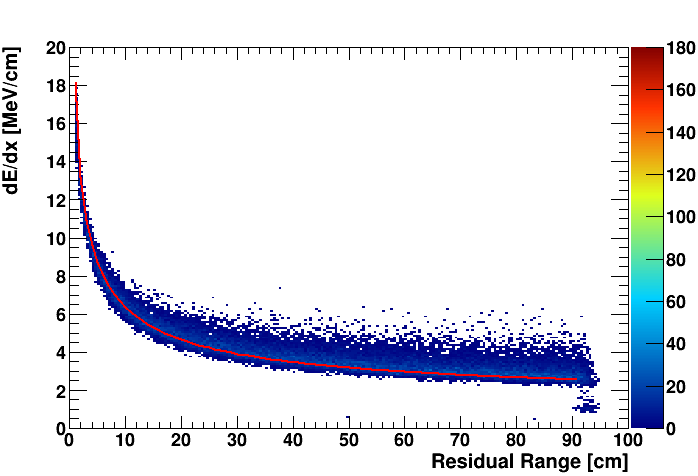
\includegraphics[width=\textwidth]{derr_proton_delta_700um}
            \caption{700 $\mu$m and delta rays included}%
            \label{fig:derr_proton_delta_700}
        \end{subfigure}
        \hfill
        \begin{subfigure}[b]{0.495\textwidth}   
            \centering 
            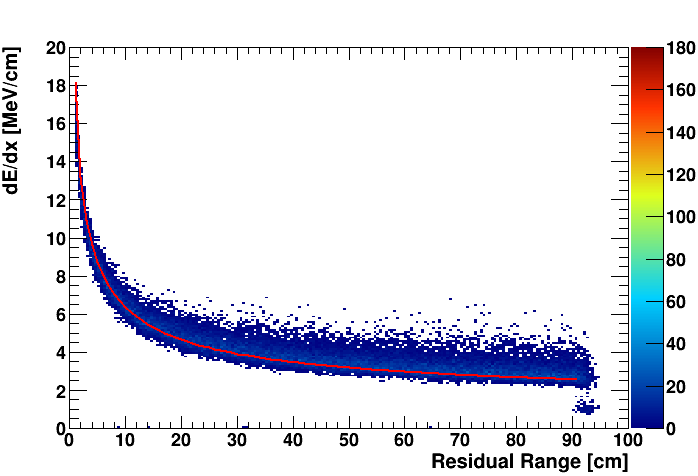
\includegraphics[width=\textwidth]{derr_proton_delta_1um}
            \caption{1 $\mu$m and delta rays included}%
            \label{fig:derr_proton_delta_1}
        \end{subfigure}
        \begin{subfigure}[b]{0.495\textwidth}   
            \centering 
            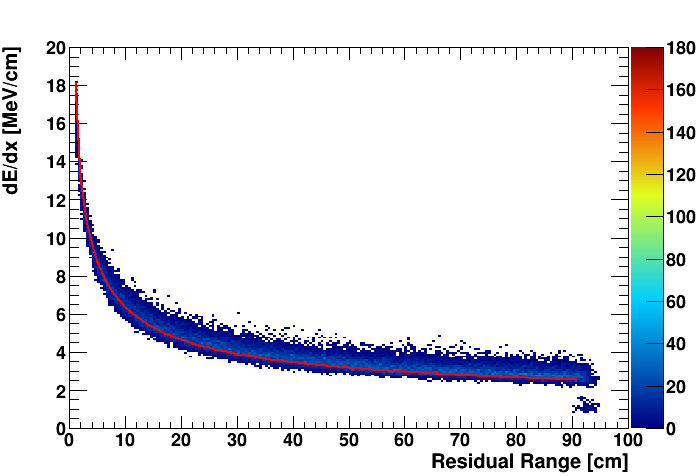
\includegraphics[width=\textwidth]{derr_proton_only_700um}
            \caption{700 $\mu$m and delta rays excluded}%
            \label{fig:derr_proton_only_700}
        \end{subfigure}
        \hfill
        \begin{subfigure}[b]{0.495\textwidth}   
            \centering 
            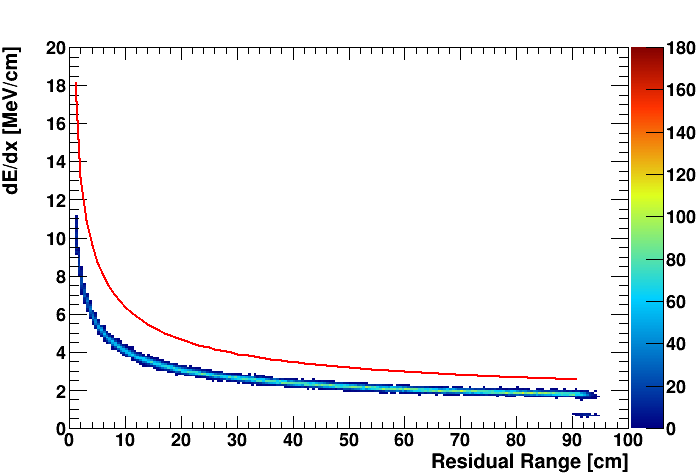
\includegraphics[width=\textwidth]{derr_proton_only_1um}
            \caption{1 $\mu$m and delta rays excluded}%
            \label{fig:derr_proton_only_1}
        \end{subfigure}
	\caption[Energy-Residual Range of Protons at Different Delta Ray Thresholds]{
	$dE/dx$ as a function of residual range for a 1 GeV proton at the delta ray threshold of 700 $\mu$m (left) and 1 $\mu$m (right), including (top) and excluding (bottom) the energy loss of delta rays. 
	}
        \label{fig:proton_derr}
\end{figure}

When delta rays are excluded in the energy loss, some noticeable effects can be seen. 
At the threshold at 700 $\mu$m, the $dE/dx$ distribution of only the primary particle but no delta rays still follows closely the Landau-Vavilov distribution, similarly to that containing both the primary particle and delta ray energy loss.
This can be seen comparing Fig. \ref{fig:derr_proton_delta_700} and Fig. \ref{fig:derr_proton_only_700} for protons, and comparing Fig. \ref{fig:derr_mu_delta_700} and \ref{fig:derr_mu_only_700} for muons. 
However, less smearing in $dE/dx$ is observed when delta rays are excluded in the energy loss, especially visible in Fig. \ref{fig:derr_mu_only_700} for muons.
At this configuration, the majority of the energy loss is carried away by the primary particle, and Geant4 already accounts for delta ray fluctuations when sampling its mean energy loss \cite{geant4}.
Introducing energy loss by delta rays only adds some additional smearing to the total $dE/dx$ distribution.

On the other hand, when the delta ray threshold is set to 1 $\mu$m and no delta rays are considered, the $dE/dx$ distribution of only the primary particle becomes narrow without any smearing and fails to follow the Landau-Vavilov distribution.
This can be seen in Fig. \ref{fig:derr_proton_only_1} for protons and Fig. \ref{fig:derr_mu_only_1} for muons. 
Isolating only the energy deposition of the primary particle is equivalent to observing a \textit{bare} proton or muon track without any delta rays produced along its path, which has not been experimentally measured before.
In this case, the stopping power distribution of the primary particle is computed by Geant4 using interpolation instead of using data-based parametrisation \cite{geant4}.
This potentially leads to inaccuracy in simulating the energy loss due to ionisation.

\begin{figure}[t!]
        \begin{subfigure}[b]{0.495\textwidth}   
            \centering 
            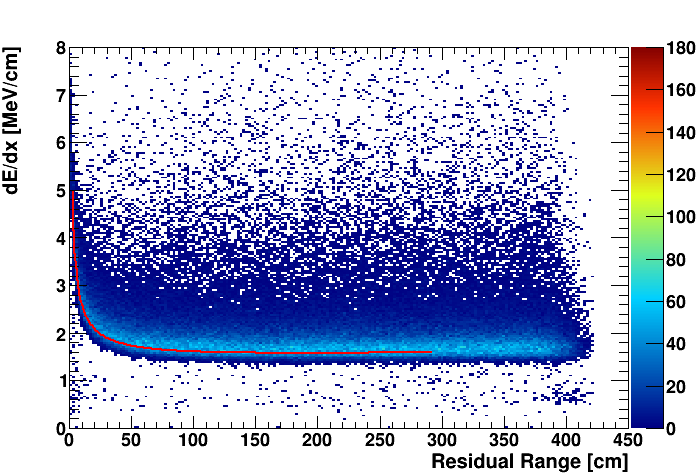
\includegraphics[width=\textwidth]{derr_mu_delta_700um}
            \caption{700 $\mu$m \\ and delta rays included}%
            \label{fig:derr_mu_delta_700}
        \end{subfigure}
        \hfill
        \begin{subfigure}[b]{0.495\textwidth}   
            \centering 
            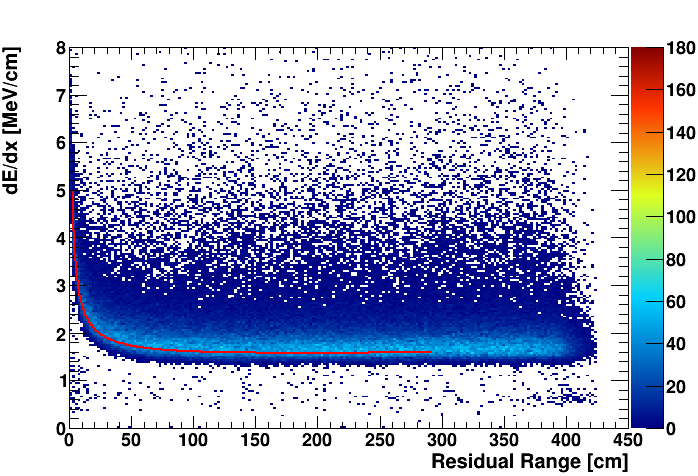
\includegraphics[width=\textwidth]{derr_mu_delta_1um}
            \caption{1 $\mu$m \\ and delta rays included}%
            \label{fig:derr_mu_delta_1}
        \end{subfigure}
        \begin{subfigure}[b]{0.495\textwidth}   
            \centering 
            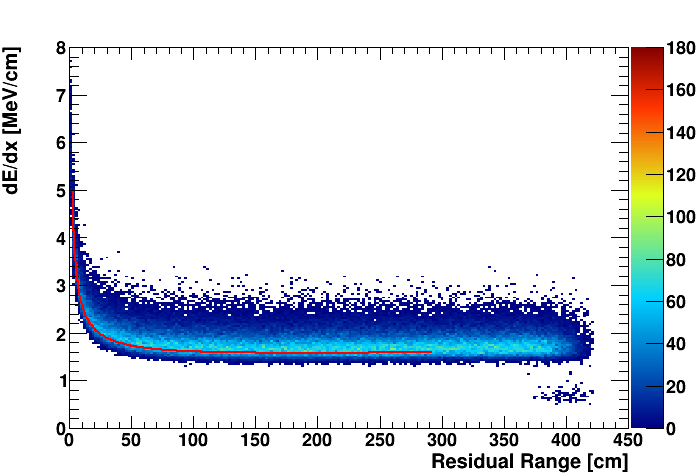
\includegraphics[width=\textwidth]{derr_mu_only_700um}
            \caption{700 $\mu$m \\ and delta rays excluded}%
            \label{fig:derr_mu_only_700}
        \end{subfigure}
        \hfill
        \begin{subfigure}[b]{0.495\textwidth}   
            \centering 
            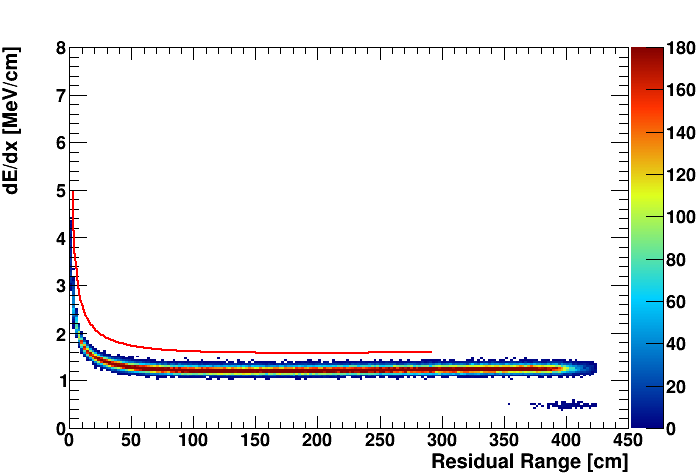
\includegraphics[width=\textwidth]{derr_mu_only_1um}
            \caption{1 $\mu$m \\ and delta rays excluded}%
            \label{fig:derr_mu_only_1}
        \end{subfigure}
        \caption[Energy-Residual Range of Muons at Different Delta Ray Thresholds]{
	$dE/dx$ as a function of residual range for a 1 GeV muon at the delta ray threshold of 700 $\mu$m (left) and 1 $\mu$m (right), including (top) and excluding (bottom) the energy loss of delta rays. 
	}
        \label{fig:mu_derr}
\end{figure}

This study demonstrates another effect of delta ray fluctuations on recombination.
Having a different $dE/dx$ to the primary particle also means that delta rays can smear the observed charge to energy loss conversion.
The amount of smearing vary differently between protons and muons, where including delta rays in the energy loss lead to more smearing in the $dE/dx$ distribution for muons than protons. 
Combining with the results from Section \ref{sec:impactDeltaRayMag}, this suggests a need for a particle-dependent recombination factor.   

%\subsection{Impacts of Step Limits}
%\label{sec:impactStepLimit}
%%Varying step limits and the effects on protons/muons
%
%The step limit study here aims to investigate the impacts of simulating a phenomenological model at a microphysics scale.
%The length $dx$, corresponding to the maximum distance the primary particle can travel per step, was studied at two configurable values: 0.3 mm and 3 mm.     
%The former is the standard value employed in the simulation workflow of SBND as well as ArgoNeuT, which is one order of magnitude smaller than the wire pitch. 
%The latter is the value of the wire pitch, which is the spatial resolution of both detectors.
%
%\begin{figure}[bp!]
%        \begin{subfigure}[b]{0.495\textwidth}   
%            \centering 
%            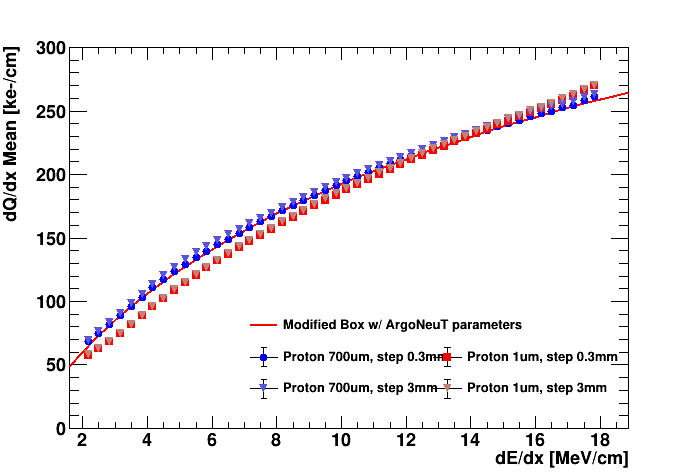
\includegraphics[width=\textwidth]{proton_profile_steplim}
%            \caption{}%
%            \label{fig:proton_steplim_magnitude}
%        \end{subfigure}
%        \hfill
%        \begin{subfigure}[b]{0.495\textwidth}   
%            \centering 
%            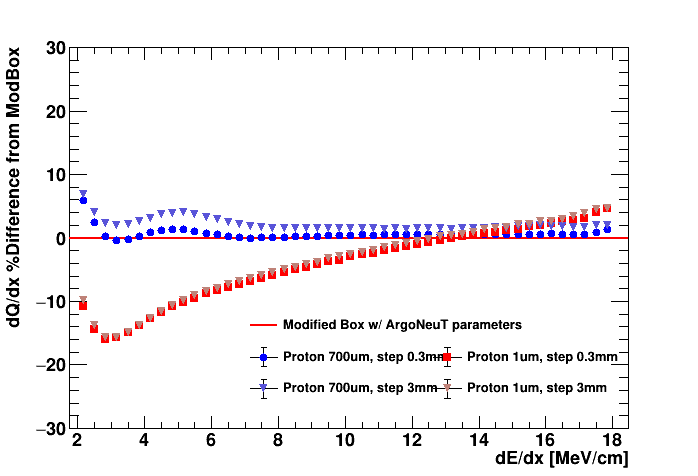
\includegraphics[width=\textwidth]{proton_profile_diff_steplim}
%            \caption{}%
%            \label{fig:proton_steplim_diff}
%        \end{subfigure}
%        \caption{Plots of the mean $dQ/dx$ (left) and its percentage difference relative to the ModBox model (right) as a function of $dE/dx$ for a 1 GeV proton, at thresholds of 700 $\mu$m and 1 $\mu$m and at step limits of 0.3 mm and 3 mm. }
%        \label{fig:proton_steplim}
%\end{figure}
%A similar analysis using the charge to energy loss conversion was employed.
%The mean $dQ/dx$ as a function of $dE/dx$ for protons and its percentage difference to the ModBox model are plotted in Fig. \ref{fig:proton_steplim}, for different combinations of step limits, 0.3 mm and 3 mm, and of thresholds, 700 $\mu$m and 1 $\mu$m.
%At the secondary production threshold of 700 $\mu$m, the increase of step limits from 0.3 to 3 mm results in an increase of the effective recombination factor across the whole range of $dE/dx$.
%The largest magnitude of the increase is between the range $dE/dx$ from 2 to 8 MeV/cm, where the majority of energy deposition occurs, and reduces with a higher value of $dE/dx$. 
%On the other hand, at the secondary production threshold of 1 $\mu$m, the effect of varying the step limit is insignificant.
%The step limit increase affects the primary particle more than the delta rays.
%This is due to the track length of the primary particle being significantly longer than that of delta rays, and therefore, more likely to propagate with a step length up to 3 mm.
%
%This result demonstrates that even though the recombination model was simulated at the observed wire pitch of 3 mm, the resulting simulation does not return the input ModBox recombination model.
%The ArgoNeuT $\alpha$ and $\beta$ parameters were tuned using a simulation with the step length $dx$ configured at 0.3 mm.
%Therefore, the simulation workflow of SBND likely only shows a good agreement when using the same configuration as ArgoNeuT.
%This shows a strong inter-dependency between the detector simulation and experimental data, particularly when it comes to tuning a phenomenological parameter for a simulation workflow.

\subsection{Recombination Studies from the ICARUS Experiment}
\label{sec:icarus}

\begin{figure}[bp!]
\centering 
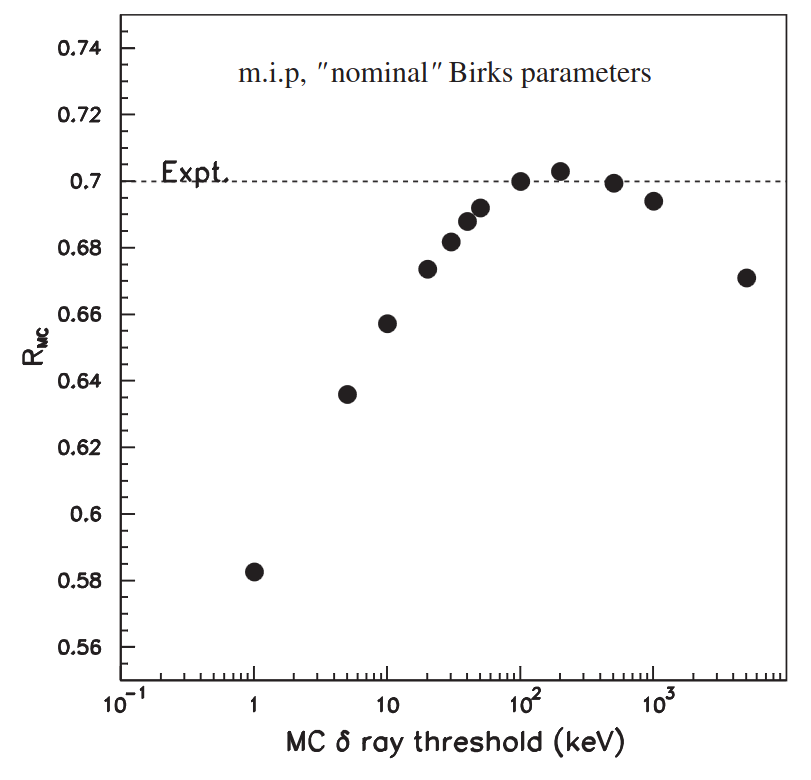
\includegraphics[width=0.5\textwidth]{icarus_recomb}
\caption[Recombination Factor Against Delta Ray Threshold]{
Recombination factor as a function of the delta ray threshold \cite{icarus_recomb}.
}
\label{fig:icarus_recomb}
\end{figure}

%ICARUS paper and why using 700 $\mu$m
%Fluctuations of delta rays influence the recombination factor.
A very similar study was carried out by the ICARUS collaboration in 2004 in Italy, to investigate delta ray fluctuations impacting recombination and also to compare against their experimental data \cite{icarus_recomb}. 
The result is shown in Fig. \ref{fig:icarus_recomb}, showing the recombination factor as a function of the delta ray threshold in MC. 
The dotted line is the expected recombination factor for a MIP muon with a KE of 250 MeV.
The recombination factor increases with the threshold and peaks at $\sim0.7$, then decreases with higher thresholds. 
This result is similar to the observation of the study described above, where the effective recombination factor reduces at small values of delta ray thresholds.

The ICARUS collaboration proposed a few different approaches toward the simulation of recombination so that delta ray fluctuations can be more accurately simulated \cite{icarus_recomb}. 
The first approach was to simulate \textit{as microscopic as possible}, by simulating delta rays with KE $\mathcal{O}$(1 eV) and range $\mathcal{O}$(10 nm).
However, they concluded that this approach was not feasible.
Firstly, the effective recombination factor of a particle always contains effects due to delta rays, and secondly, computing resources are limited.
Another proposal was an empirical approach, to choose the best delta ray threshold in simulation to reproduce the data with a reasonable computing consumption.
This number was found to be 3 $\mu$m, equivalent to simulating delta rays having a KE as low as 10 keV.

%TODO: Check Gray's paper on recombination dependence of track angular

%gain more understanding in recombination : angular dependency
%TODO: add ref recombination dependence on angular
Also recently from the ICARUS collaboration, now with the detector relocated to Fermilab, a study in 2024 of recombination showed a clear dependence of recombination on the angle of the particle track to the drift electric field \cite{elipsoid_recomb}.
An ellipsoidal modification to the ModBox recombination model was proposed and able to describe the data across all measured angles. 
This result has significantly improved the observed charge to energy loss conversion of a particle, which is critical for particle identification of an LArTPC.   

These results from the ICARUS collaboration have collectively enhanced the understanding of recombination, as well as guided how to model recombination at SBND.
In the scope of calibrating the SBND detector, it is highly recommended to follow a data-driven approach such that the simulation of delta rays and recombination should be tuned to best match the observed data, as done by earlier experiments like ICARUS and ArgoNeuT.

\section{Concluding Remarks}
\label{sec:concludeDeltaRay}

Two studies within the scope of calibrating ionisation electron signals were presented. 
The first study describes a procedure to measure the electron lifetime using anode-to-cathode crossing cosmic muons and quantify biases in the acquired lifetime due to SCE and diffusion. 
The second study examines the simulation of delta rays and recombination, and how delta ray fluctuations can impact the effective recombination factor and consequently, the charge to energy loss conversion of a particle.
These studies help understanding how different detector effects and physics processes can impact the charge depositions on wires, which can be pinned down and corrected for.
This calibration process necessitates high precision measurements, which are essential for any physics analysis at SBND, including the search for HNLs.
The following Chapter \ref{ChapterSelect} focuses on the selection of HNLs, of which many reconstruction variables describing the calorimetry and topology of a particle relies on having an accurate charge information. 

%This simulated study demonstrates a strong inter-dependency between detector simulation and data and therefore, the accuracy of the recombination factor can be improved by using parameters tuned to data measured by SBND.
%Moreover, the study shows a distinct difference in recombination between proton and muon and perhaps suggests a need for a particle-dependent model.
%Modelling recombination for a specific sample of particle type is feasible with the large statistics of SBND. 
%This will allow for constructing a particle-dependent recombination factor that can be directly input into LArG4.
